\documentclass[a4paper]{article}

\usepackage{listings}
\usepackage{graphicx}
\usepackage{fancyhdr}
\usepackage{color}
\usepackage{xcolor}
\pagestyle{fancy}

\lhead{Tube Tracker}
\rhead{CSN08113}
\lfoot{Final Report}
\cfoot{\thepage}
\rfoot{Gareth Pulham, 40099603}

\lstdefinestyle{customc}{
    belowcaptionskip=1\baselineskip,
    frame=single,
    xleftmargin=\parindent,
    language=C,
    showstringspaces=false,
    basicstyle=\footnotesize\ttfamily,
    keywordstyle=\bfseries\color{green!40!black},
    commentstyle=\itshape\color{purple!40!black},
    identifierstyle=\color{blue},
    stringstyle=\color{orange},
}


\begin{document}
    \begin{titlepage}
        \title{Physical Computing CSN08113\\
            Tube Tracker
        }
        \author{Gareth Pulham, 40099603}
        \date{\today}
        \maketitle
        \thispagestyle{empty}

        \begin{abstract}
            This project aims to produce a ``Tube Tracker'', a device which can be used to identify the location of a catheter inside the body by detecting the metal guide wire when placing it.
            To do so, the device interprets signals produced by a COTS metal detector commonly used for security purposes.

            By examining and measuring the metal detectors internal construction, it was possible to identify and interpret the strength of metal detection, which can then be displayed to the user to deduce the location of the guide wire.

            As a result of this work, a working prototype was developed and demonstrated.

            This project was undertaken in partnership with Megan Currie, a product design student at Edinburgh Napier University, who developed the concept and packaging for this project.
        \end{abstract}
    \end{titlepage}

    \tableofcontents

    \section{Introduction}
    Surgery and other clinical procedures are under ever increasing pressure to be able to up their effectiveness, complete more radical and effective procedures, and treat previously unreachable parts of the body, while at the same time continuously decrease their invasiveness and other adverse impacts on the patient. These pressures have led to continous innovation in medical technology, with one of the most significant jumps being the introduction of laparoscopy, also known as keyhole surgery, where only a tiny incision is made, and all tools are operated on flexible stalks passed through this small hole, with navigation being done by camera.

    There are other instances in the clinical setting where we want to execute minimally invasive procedures, and have to accept that this means a more challenging working environment, such as not being able to see the tools in use, and a subfield of computer-assisted surgery, `surgical navigation', has sprung up around this, providing better insight into the position and manoeuvring of tools.

    This project aims to be the first part of a wider ``Swiss Army Nurse'' project, a collection of many useful nursing tools in a handheld package. This component is a simple navigation tool to help nurses identify the location of a catheter as it's being inserted, a simple procedure but which requires some practice in inexperienced nurses to ensure that the tube follows the correct path as it's being inserted.

    \section{Deliverables}
    \begin{itemize}
        \item Prototype Tube Tracker
        \item Final Report (this document)
    \end{itemize}

    \section{Design}
        \subsection{Sensor Types}
        The mode of operation of medical navigation falls into five broad categories:
        \begin{itemize}
            \item Optical
            \item Electromechanical
            \item Electromagnetic
            \item Ultrasonic
            \item and Radiological
        \end{itemize}
        For the purposes of this project, radiological sensing is not considered a viable option due to it's highly controlled distribution and the impact it has on patients and operators, amongst other reasons.

        An optically guided solution would also not be suitable for this project, as it depends on a number of preparatory steps, such as registering a 3D model of the operating area. Additionally, they are most effective with rigid tools, unlike the catheter that this project aims to use.

        This leaves three remaining options: ultrasonic, electromagnetic, and electromechanical.

            \subsubsection{Ultrasonic}
            Ultrasonic sensing relies on sending high frequency sound ``chirps'' into the body, and then analysing the echos reflected by tissue structures or other objects that the chirps strike. It has a proven track record, and is used daily in a range of settings, from routine obstretic imaging to emergency medical teams providing trauma care.

            Ultrasound also has a relatively low training cost compared to other sensing methods such as radiological and optical, but it does have overhead in preparing a patient for imaging - the area where the image is to be taken must be cleared of obstructions (dirt, hair, etc) and the application of gel to improve conductivity.

            The real challenge to implement ultrasonic in this project is however is that ultrasound requires sophisiticated signal processing capabilities to turn the returned echoes into an understandable image. Additionally, it will be difficult to differentiate the catheter from other body tissues (searching for a metal wire behind the sternum\slash in front of the spine, inside of an airspace).

            \subsubsection{Electromagnetic}
            Electromagnetic sensing in this instance would be possible as we are essentially operating as a metal detector to find the guidewire inserted into the catheter. Some of the advantages here are that the device would be very simple to design, develop, and use. With this mode of sensing, the device would offer a signal strength as it passed over the metal wire in the catheter. To use, the operator simply needs to move the device over the body until they can identify the point of maximum signal strength.

            However, electromagnetic does have some downsides as well. The most notable of these are the calibration that they require to get the best results and maximum swing over the entire scale when moving over metal. Another is that their use could be contraindicated in patients who have pacemakes. An example of this already in real life is the separate screening queue at airports and other transport hubs where full body metal detectors are used.

            \subsubsection{Electromechanical}
            Electromechanical navigation is where the catheter tip can be instrumented with accelerometers/gyros, and we can measure the motion recorded on these the same way as used in INS. By continually integrating these accelerations over time we can get speed, and integrating again gives us a displacement from where the measurements were started.

            Again there are downsides to this method, in particular, single-use elements have to be instrumented with expensive parts which then cannot be reused. Additionally, like optical systems, for the best results, the area where the device will be used should be pre-registered.

        \subsection{High Level design}
        The choice was made to work with Electromagnetic sensors, as for the purposes and scope of this project, it offers acceptable accuracy and usability with a very low complexity to implement. The high level block diagram for the system is shown below.
        \begin{figure}[h]
            \centering
            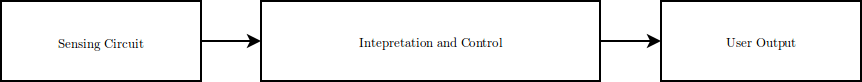
\includegraphics[width=0.75\textwidth]{images/highlevel}
            \caption{High level design showing Input, Processing, and Output components.}
        \end{figure}

        Following this design it was easy to attack each section of the project as an individual module, focussing separarely on each and identifying how best to interface between them.

    \section{Implementation}
        \subsection{Input - Sensing system}
        After deciding to use an electromagnetic sensing system as part of the system design, further research at this stage was called for to find out more about previous study of the effectiveness of different methods.
        This research found several studies that trialled using simple handheld metal detectors to identify foreign bodies swallowed by children(!!!).
        Being able to use COTS parts such as airport-style metal detectors was a major boon as this drastically reduced the complexity of what needed to be implemented specifically for this project.

        This complexity is however instead swapped out for the need to reverse engineer an otherwise closed system to get the information needed to present the user with a reading - and this is where the majority of the time used implementing this project was spent.

        After time spent inspecting the PCB of the metal detector visually and electrically (with the aid of simple tools, such as a multimeter and an oscilloscope), the following subsystems were indentified:
        \begin{itemize}
            \item RF oscillator
            \item RF coil
            \item RF signal conditioner (processing of the RF signal to a more usable analogue value)
            \item Logical signal conditioner (processing the analogue value from above to produce logical outputs)
            \item Output handling (RG LED and selection between buzzer/pager motor and drivers for those)
            \item Power supply
        \end{itemize}

        Once these systems had been identified, the main target for further investigation was the logical signal conditioning circuit, which analysed a roughly processed signal from the RF units and identified whether or not the devices alert should be triggered.
        Several points inside this system were individually investigated to gain an understanding of what steps were applied between input and output. Notably these steps were additionally smoothing, autothresholding, and comparison to a fixed reference voltage.
        
        Initially, the project tried to simply read the output of this unit, however the detector applies a kind of autothresholding process so that the signal strength fed to the comparator decayed over time.
        This is likely so that the device stays responsive across a wide range of changing environments - in essence, avoiding the device becoming useless in environments that are simply more conducive to strongly received signals.
        Additionally, it means that the operator would not have to manually calibrate to address these changes.

        While this is advantageous in simple usages searching for detection/no detection, this project is less concerned about thresholding and more about allowing a user to manually interpret a partially processed signal strength - it would not do well for the device to ``lose'' the signal simply because it wasn't being moved fast enough.
        Because of this, our device instead taps into the connection between the smoothing and autothresholding portions. This signal was found to vary from 2.1V when no metal was placed near the RF coil, to 1.8V when a large piece of metal was placed directly on top of it.
        From here, it was relatively simple so read this with our devices ADC and display a different readout across this range.

        \subsection{Process - Interpretation signal and control of output}
        Now that a target had been identified and understood, it was possible to develop a microcontroller ($\mu$C) program to interpret readings and display the correct output.

        The $\mu$C selected for this job is the Atmel AVR ATmega328P. A staple in the hobbyist world, this is the device that provides the brains to the ``Arduino'' development and learning board. While this project did not use an Arduino, this device provided the right features required - most importantly, an analogue to digital converter to digitise the signal read for mathematical comparison.

        The program written was extremely simple, setting up the ADC to read and digitise the signal, and based on this signals level, light an increasing number of LEDs to indicate stronger signal, and therefore the tube tracker being closer to the catheter's guidewire.
       
        \subsubsection{Source listing for the Tube Tracker prototype}
        \lstinputlisting[style=customc]{../src/tracker.c}

        \subsection{Output - LED signal strength}
        The output for this device was required to be straightforward and highly visible, as well as reliable.

        There are many options for displaying signal strength outputs. For the purposes of this project, two were considered:
        \begin{itemize}
            \item Analgoue dials - very intuitive description, and capable of showing the full range of values rather than quantising to a smaller number of steps. However, these displays are also power hungry, and easily affected by motion and magnetic fields.
            \item LEDs - clear in all conditions, and not affected bu the environment in the same way physical dials are. However the force the application to quantise the signal strength and as such there's a loss in resolution.
        \end{itemize}

        Ultimately, the LEDs were chosen to be the display for the tube tracker. In addition to the above points, they are very robust and unlikely to be damaged if the device is dropped. It was felt that the loss in resolution compared to an analogue display was not so bad that the devices usability would be compromised.

        \subsection{Overall design output}
        \begin{figure}[h]
            \centering
            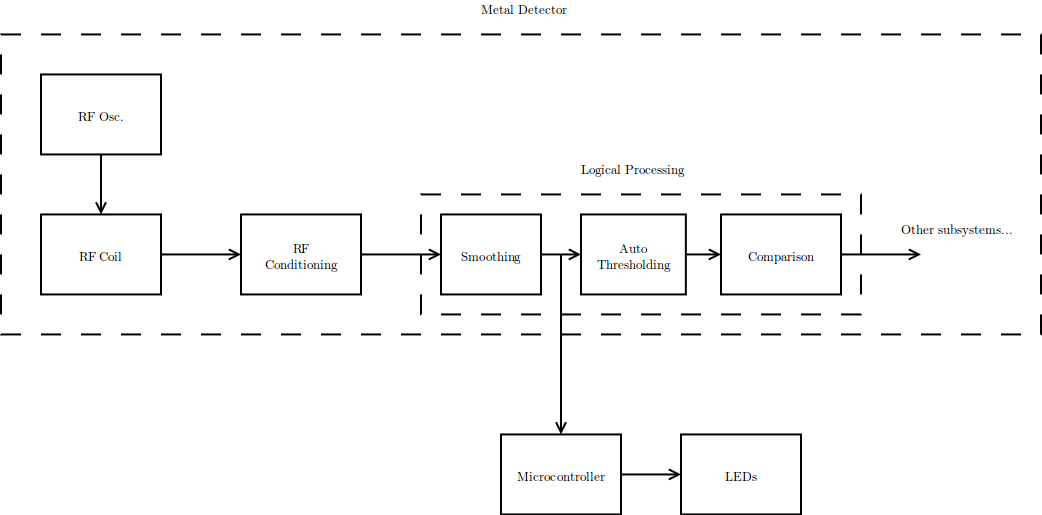
\includegraphics[width=\textwidth]{images/complete.png}
            \caption{The complete system diagram showing components relevant to the project}
        \end{figure}


    \section{Schematic}
    \begin{figure}[h]
        \centering
        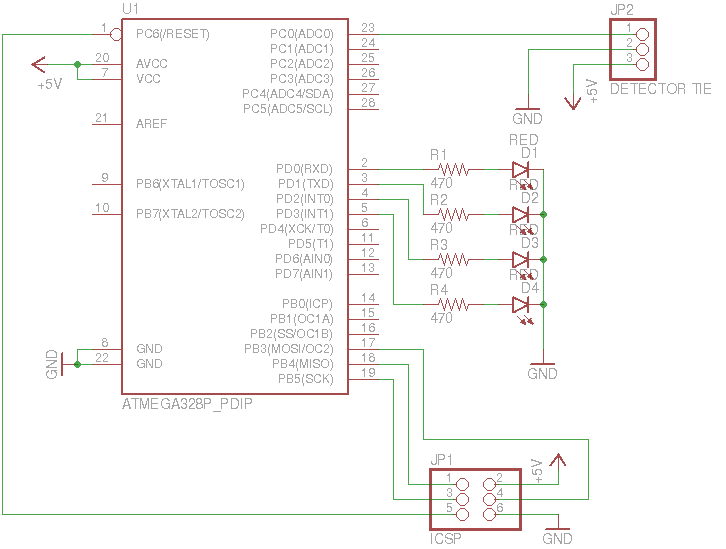
\includegraphics[width=0.75\textwidth]{images/schematic}
        \caption{The schematics of the implemented prototype}
    \end{figure}

\end{document}
